% !TEX TS-program = pdflatex
% !TEX encoding = UTF-8 Unicode

% This is a simple template for a LaTeX document using the "article" class.
% See "book", "report", "letter" for other types of document.

\documentclass[11pt]{article} % use larger type; default would be 10pt

\usepackage[utf8]{inputenc} % set input encoding (not needed with XeLaTeX)

%%% Examples of Article customizations
% These packages are optional, depending whether you want the features they provide.
% See the LaTeX Companion or other references for full information.

%%% PAGE DIMENSIONS
\usepackage{geometry} % to change the page dimensions
\geometry{a4paper} % or letterpaper (US) or a5paper or

\usepackage{graphicx} % support the \includegraphics command and options

% \usepackage[parfill]{parskip} % Activate to begin paragraphs with an empty line rather than an indent

%%% PACKAGES
\usepackage{booktabs} % for much better looking tables
\usepackage{array} % for better arrays (eg matrices) in maths
\usepackage{paralist} % very flexible & customisable lists (eg. enumerate/itemize, etc.)
\usepackage{verbatim} % adds environment for commenting out blocks of text & for better verbatim
\usepackage{subfig} % make it possible to include more than one captioned figure/table in a single float
% These packages are all incorporated in the memoir class to one degree or another...
\usepackage{amsmath,epsfig}
\usepackage{amsthm, amssymb}

%%% HEADERS & FOOTERS
\usepackage{fancyhdr} % This should be set AFTER setting up the page geometry
\pagestyle{fancy} % options: empty , plain , fancy
\renewcommand{\headrulewidth}{0pt} % customise the layout...
\lhead{}\chead{}\rhead{}
\lfoot{}\cfoot{\thepage}\rfoot{}

%%% SECTION TITLE APPEARANCE
\usepackage{sectsty}
\allsectionsfont{\sffamily\mdseries\upshape} % (See the fntguide.pdf for font help)
% (This matches ConTeXt defaults)

%%% ToC (table of contents) APPEARANCE
\usepackage[nottoc,notlof,notlot]{tocbibind} % Put the bibliography in the ToC
\usepackage[titles,subfigure]{tocloft} % Alter the style of the Table of Contents
\renewcommand{\cftsecfont}{\rmfamily\mdseries\upshape}
\renewcommand{\cftsecpagefont}{\rmfamily\mdseries\upshape} % No bold!

\usepackage{ textcomp }

%%% END Article customizations


%%% The "real" document content comes below...

\title{LING773 - Negotiations Project Report}
\author{Peng Ye, Youngil Kim, Olivia Buzek}
%\date{} % Activate to display a given date or no date (if empty),
         % otherwise the current date is printed

\begin{document}
\maketitle


\section{Introduction}

The members of this group are Peng Ye, Youngil Kim, and Olivia Buzek.

\section{Preprocessing}

The data was lowercased, punctuation removed, with non-ASCII characters removed, and tokenized using Treebank tokenization rules.  Misspellings were not corrected.  In these experiments, we restricted ourselves to the 60 dyads for which a joint profit was reported in the original Imai and Gelfand work.

\section{Feature extraction}
In this section, we will introduce three types of features that are extracted for predicting joint-profit.
\subsection{Meta information}

The meta-data features used were the same as those originally used in the Imai and Gelfand experiment.

\subsection{Code-based N-Gram feature}
The dataset is annotated by thought unit with a code representing the function of that thought unit in the discussion.  Some code indicates positive interaction between speakers, for example, 'RP' means positive reaction; some code indicates negative interaction, for example, 'RN' means negative reaction. Intuitively, negative or positive interaction should have high correlation with joint profit, thus thought unit code is informative feature for predicting joint profit. The second type of feature we use is though unit code based feature. Considering a dyad as a sequence of codes, we then extract code-based unigrams and bigrams as our features. Specifically, for each dyad we extract the following features:
\begin{itemize}
\item Unigram based features:
\begin{itemize}
\item Overall features: (Overall features are extracted from the entire dyad.)

      number of total thought units, number of thought units of each code, percentage of thought units of each code
\item Wine features: (Wine features are extracted from wine part of the dyad)

      number of total thought units (in wine part), number of thought units of each code, percentage of thought units of each code

\item Grocery features: (Grocery features are extracted from grocery part of the dyad)

number of total thought units (in grocery part), number of thought units of each code, percentage of thought units of each annotation

\item Relative feature: Relative feature indicates the difference between wine part and grocery part of the dyad.

J-S divergence between the unigram distribution over wine dialog and unigram distribution over grocery dialog
\end{itemize}
\item Bigram based features:
\begin{itemize}
\item Overall features: (Overall features are extracted from the entire dyad.)

      number of turns (change of speakers) in the dyad, number of code-based bigram, percentage of code-based bigram
\item Wine features: (Wine features are extracted from wine part of the dyad)

      number of code-based bigram, percentage of code-based bigram
\item Grocery features: (Grocery features are extracted from grocery part of the dyad)

      number of code-based bigram, percentage of code-based bigram
\item Turning point features: A turning point in a dyad is where the speaker changes. Features extracted at turning points indicate how one speaker respond the other speaker.

      number of code-based bigram, percentage of code-based bigram

\item Relative feature:

      J-S divergence between the bigram distribution over wine dialog and bigram distribution over grocery dialog
\end{itemize}
\end{itemize}

In our corpus, we have 38 code-based unigrams and 660 code-based bigrams. We extract a total of 5515 code-based features from each dyad.

We chose to use bigrams as well as unigrams for the code-based features, because it seemed likely that a sequence of events would be more informative than just the instance of an event in the course of a negotiation.

It is worth noting that features introduced above are redundant, for example the percentage of a unigram and the number of times a unigram occurred are correlated with each other and are only different by a constant factor.  In our initial feature extraction, we do not eliminate those redundant features.  Instead, we collect as many features as possible and perform feature selection on these features to choose the most informative features. Feature selection will be illustrated in detail in the next section.

\subsection{Word-based N-Gram feature}
We extract word-based n-grams through following process.
\begin{itemize}
\item Preprocessing with raw data - creating \textit{fields\_speaker.txt}: \newline
We analyzed \textit{merged\_turns.csv} and \textit{metadata.csv} for creating \textit{fields\_speaker.txt} file. Because some dialogues do not have \textit{joint profit} in \textit{metadata.csv} file, we should rule out those dialogues even though they exist in \textit{merged\_turns.csv} file. In addition, we rearranged the sequence of fields for better readability.  The dyid is now positioned as the first item.

\item Count n-grams and Create n-gram ID:\newline
After tokenizing, we count number of n-grams to see the characteristics of each dialogue. To counting ngrams, we used \textit{count.pl} in Ted Pedersen Ngram Statics Package with general stop words, since stop words are likely not informative. We separately count n-grams for Wine, Grocery, and all dialogues for seeing the characteristics of each group of speakers. N-grams were also computed for each dyad. \newline
In addition, we created n-gram id files to express ngrams. For example, \textit{grand opening date} which is one of trigram is expressed as \textit{3-0001}. By using this ngram id, we can save memory and storage for analyzing whole data.
\item Make n-gram feature file:\newline
By using counted n-grams, we created n-gram feature file which can be converted into an ARFF format, input format of Weka. Each row in the file contains n-gram information of each dyad. The first column shows the \textit{dyID}, and the following colums show ngram id and the number of ngrams in the dialogues. Following example shows a part of the feature file.
\begin{itemize}
\item Example
\begin{verbatim}
02,1-0002:30,1-0001:23,1-0040:18,1-0009:16,1-0012:15 ... ...
03,1-0006:30,1-0001:29,1-0048:23,1-0026:21,1-0025:20 ... ...
\end{verbatim}
\end{itemize}
We made three n-gram feature files for each category, Wine, Grocery, and all dialogues.
\end{itemize}

In our experiment, we actually used only the n-gram extracted from entire dyad only. We have a total of 5754 word-based ngram features.

\section{Regression}
\subsection{Feature Selection}
\label{sec:fv_selection}
Feature subset selection is a process of identifying the most informative features and removing irrelevant and redundant features. In our experiment, we extracted a large number of features.  To decrease the time it would take to train, and to find out what the most useful features were, we used a feature selection process. In Weka, we use 'BestFirst' as the search method and use 'CfsSubsetEval' as the attribute evaluator to finding the most informative features. As is explained in Weka, 'CfsSubsetEval' evaluates ``the worth of a subset of attributes by considering the individual predictive ability of each feature along with the degree of redundancy between them'' and 'BestFirst' searches ``the space of attribute subsets by greedy hillclimbing augmented with a backtracking facility. Setting the number of consecutive non-improving nodes allowed controls the level of backtracking done.'' In our experiment, the best first search started with the full set of attributes and searched backward. The top ten best word-based n-gram features are shown in Table.\ref{tab:selected_ngram} and the top ten best code based ngram feature is shown in Table. In this table, ``percentage-of-(MIN-QR)-turns'' means the percentage of the bigram of MIN-QR extracted from turning points of a dyad, where the conversation switches from one speaker to the other.
\begin{table}
  \centering
  \caption{THE TOP TEN MOST INFORMATIVE WORD-BASED AND CODE-BASED NGRAM FEATURE}
  \begin{tabular}{|c|c|}
     \hline
CODE-BASED NGRAM FEATURE & WORD-BASED NGRAM \\
  \hline
percentage-of-(MIN-QR)-turns & hours \\

percentage-of-(SF)-overall & special\\

percentage-of-(SF)-grocery & great\\

number-of-(IR)-overall & 30k\\

percentage-of-(SBR-SF)-overall & agreeable\\

percentage-of-(OM-QM)-wine & 630\\

percentage-of-(MIN-IR)-wine & 1030pm\\

percentage-of-(IP-SF)-grocery & luxurious\\

percentage-of-(IP-IDN)-turn & people work\\

percentage-of-(IDN-SBR)-turns & crust grocery\\
  \hline
  \end{tabular}\label{tab:selected_ngram}
\end{table}

We extract the top 20 most informative code-based features and word-based feature, together with features extracted from meta information as the final feature. Specifically, we have a total of 49 features for each of the 61 dyads. It should be noted that feature selection performed on all the available data may lead to overfitting.  Thus, we first perform feature selection on all data to see which features are the best for our current dataset. In the following experiments, we split the dataset into training and testing sets, and select features only from the training set.

\subsection{Regression Algorithms}
We used three different types of regression methods provided in Weka for predicting joint profit.
\begin{itemize}
\item weka.classifiers.functions.SMOreg: support vector machine for regression, and we use RBF kernel. \cite{SVM} \cite{SMO}
\item weka.classifiers.functions.LinearRegression: using linear regression for prediction.
\item weka.classifiers.meta.Bagging + weka.classifiers.trees.REPTree: bagging predictor based on REPTree which builds a regression tree using information gain. \cite{bagging}
\end{itemize}

\subsection{Evaluation Metrics}
The following metrics are used to evaluate the proposed method.

\begin{enumerate}
\item Correlation coefficient (CC)

\item Mean absolute error (MAE)

\item Root mean squared error (RMSE)

\item Relative absolute error (RAE)

\item Root relative squared error (RRSE)
\end{enumerate}

\section{Experiment results}
In this section, we will show the experimental results using the features obtained through the feature selection process and the three different regression methods. This result is compared to a baseline experiment, where code-based unigram features and meta information are directly used to form a 241-by-1 feature vector (without further feature selection process) for each dyad. Our experimental results show that using those selected features, we can achieve better performance. We did two experiments:

\begin{itemize}[1)]

\item In the first experiment, the improved method uses feature obtained by running feature selection on the entire dataset and it is compared to baseline method described above. As is shown in Table \ref{tab:result1} and Table \ref{tab:result2}, the improved method consistently performs better than the baseline method when use SVM for regression. Compared to the linear regression and bagging methods, SVM regression provided more consistent and better performance.

\begin{table}
  \centering
  \caption{EXPERIMENT RESULTS WITH TEN FOLD CROSS-VALIDATION AND FEATURE SELECTION PERFORMED ON ALL DATA}
  \begin{tabular}{|c|c|c|c|c|c|c|}
     \hline
         &       & CC & MAE & RMSE & RAE & RRSE\\
     \hline
     SVM & Baseline & 0.72  & 57.93  & 74.01  & 64.90\%  & 70.44\%\\
         & Improved & \textbf{0.90}  & \textbf{43.03}  & \textbf{53.25}  & \textbf{48.20\%}  & \textbf{50.68\%}\\
     \hline
  Linear & Baseline &  0.71 & 64.32  & 86.42  & 72.05\% & 82.25\%\\
  Regression & Improved & 0.76  & 69.30  & 88.11  & 77.63\%  & 83.87\%  \\
  \hline
  REPTree & Baseline &  0.66 & 67.75  & 81.42  & 75.89\%  & 77.50\%\\
  Bagging & Improved &  0.69 & 64.16  & 77.01  & 71.87\%  & 73.49\%\\
  \hline
  \end{tabular}\label{tab:result1}
\end{table}

\begin{table}
  \centering
  \caption{EXPERIMENT RESULTS WITH FIVE FOLD CROSS-VALIDATION AND FEATURE SELECTION PERFORMED ON ALL DATA}
  \begin{tabular}{|c|c|c|c|c|c|c|}
     \hline
         &       & CC & MAE & RMSE & RAE & RRSE\\
     \hline
     SVM & Baseline & 0.68  & 66.33  & 83.57  & 74.15\%  & 79.63\%\\
         & Improved & \textbf{0.89}  & \textbf{44.31 } & \textbf{54.41}  & \textbf{49.53\% } & \textbf{51.85\%}\\
     \hline
  Linear & Baseline &  0.67 & 70.47  & 90.95  & 78.77\% & 86.67\%\\
  Regression & Improved & 0.53 & 82.82 & 105.08  & 92.58\%  & 100.13\%  \\
  \hline
  REPTree & Baseline &  0.51 & 73.06  & 89.84  & 81.67\%  & 85.61\%\\
  Bagging & Improved &  0.69 & 62.44  & 78.01  & 69.80\%  & 74.34\%\\
  \hline
  \end{tabular}\label{tab:result2}
\end{table}

\item In the second experiment, we first split our dataset into training and testing set, where in training set we have 46 dyads and in testing set, we have 15 dyads. We split the dataset in a way such that the distribution of the value of joint profit is ``uniform'' in both training and testing set.
We then perform the feature selection procedure mentioned in Section \ref{sec:fv_selection} on training set. The classifier training is also performed solely on training set. We then test the trained model on our testing set.

In this experiment, we only used SVM regression and obtained the following result:

\begin{table}
  \centering
  \caption{EXPERIMENT RESULTS FEATURE SELECTION PERFORMED ON TRAINING DATA}
  \begin{tabular}{|c|c|c|c|c|c|c|}
     \hline
         &       & CC & MAE & RMSE & RAE & RRSE\\
     \hline
     SVM & Baseline (5-fold c-v)& 0.68  & 66.33  & 83.57  & 74.15\%  & 79.63\%\\
         & Improved & \textbf{0.76}  & \textbf{61.54 } & \textbf{71.58}  & \textbf{69.65\% } & \textbf{68.69\%}\\
  \hline
  \end{tabular}\label{tab:result3}
\end{table}

This result should be compared with the five fold cross-validation result of baseline method. As is shown in Table \ref{tab:result3}, although our improved approach still performs better than the baseline approach.

\end{itemize}

\section{Analysis}

Using all of the regression methods, except when using 5-fold cross validation and linear regression, the selection of features from the wider set developed in this project performed better than any of the baseline experiments, which only considered the metadata features and a simple code-based unigram feature set to represent each dyad.  Using Support Vector Machines led to the most consistently sizable improvement, whether using 10-fold or 5-fold validation.

The use of SVM and this feature selection method makes it possible to predict the joint profit with a correlation of 0.9.  Interestingly, the most informative features for predicting the joint profit involved sequences of mostly factual statements, neutral-tone comments of various kinds, rational argument and statements of priorities.  None of the thought unit codes involving emotion, persuasion or positive / negative tone were very informative for correlation, nor were thought unit codes that had to do with disagreement, making concessions, or off-topic comments.  Consider the most informative feature, percentage-of-(MIN-QR)-turns, referring to the sequence of a general on-task related statement in a neutral tone by one individual, followed by a question about the individual's priorities from the other participant.  Like the rest of the informative features, this feature shows a rational, on-topic, focused discussion.  This suggests that the best way to determine if a negotiation will succeed is by examining how much of their conversation was conducted as a rational discussion.

The weights for the informative features under SVM regression can be seen in Table \ref{tab:ftr_weights}.

\begin{table}
  \centering
  \caption{THE TOP TEN MOST INFORMATIVE WORD-BASED AND CODE-BASED NGRAM FEATURE}
  \begin{tabular}{|c|c| c | c|}
     \hline
NEGATIVE & WEIGHT & POSITIVE & WEIGHT \\
  \hline
percentage-of-(IP-SF)-grocery & -0.116 & 1-0020 (hours) & 0.2806 \\
number-of-(IS)-grocery & -0.1193 & percentage-of-(OM)-grocery & 0.2691 \\
cultural_intelligence & -0.1652 & 1-1800 (luxurious) & 0.2121 \\
openness & -0.1705 & 1-0091 (pretty) & 0.1656 \\
percentage-of-(SBR-SF)-overall & -0.1726 & percentage-of-(MIN-IR)-wine & 0.1561 \\
percentage-of-(IDN-SBR)-turns & -0.1861 & 1-0090 (great) & 0.1385 \\
1-0483 (drinks) & -0.2473 & percentage-of-(MIN-QR)-turns & 0.1314 \\
percentage-of-(SF)-overall & -0.2476 & extroversion & 0.1095 \\
1-0177 (low) & -0.3044 & 2-0004 (renovation costs ) & 0.1047 \\
percentage-of-(IP)-overall & -0.3816 & & \\
  \hline
  \end{tabular}\label{tab:ftr_weights}
\end{table}

From this, we can see that, as Imai and Gelfand discovered, cultural intelligence and openness had little to do with a successful negotiation.  In fact, we see instead that the sorts of statements made seemed to have more bearing on success, as well as which words were used, to a degree.  The unigrams which contributed to success seemed to have to do with expressing convincing or positive emotions (luxurious, pretty, great), or simple facts (hours, renovation costs).  The only metadata feature which contributed was extroversion.  (It is possible that in this experiment, task-related words such as ``drinks", ``hours", and others should have been treated as stop-words, given that almost every dyad could easily contain those words.)  Also seemingly contributing to success was talking about agreement and priorities: ``OM" refers to having secure agreement; ``IR" to providing information about priorities; and ``QR" to a question about priorities.  The neutral emotions and factual statements expressed in a high percentage contributed negatively to success.

% \begin{tabular}{ c c }
\begin{figure}
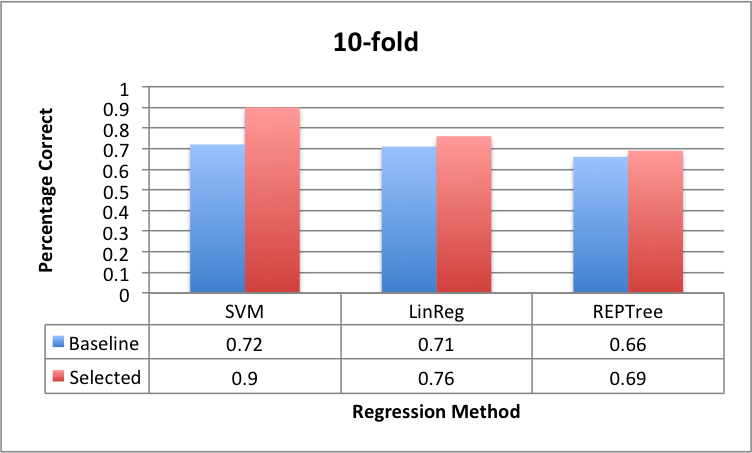
\includegraphics{../results/10fold.png}
\caption{Results from 10-fold cross-validation.}
\end{figure}
%&
\begin{figure}
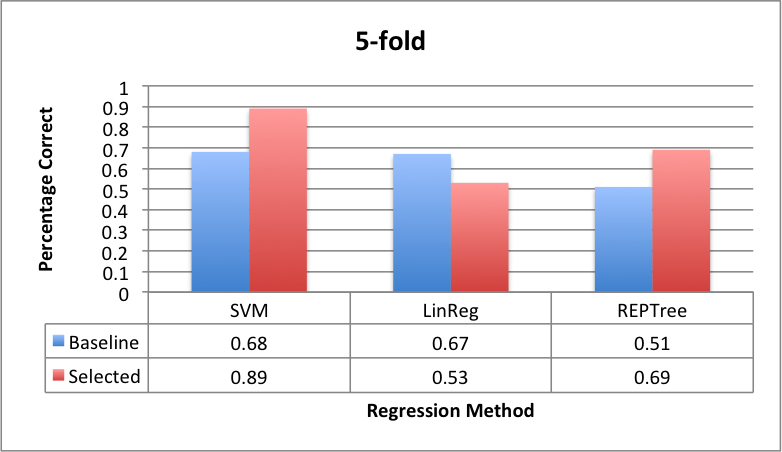
\includegraphics{../results/5fold.png}
\caption{Results from 5-fold cross-validation.}
\end{figure}
% \end{tabular}

\section{Conclusions}

We can draw two sets of conclusions from this experiment.  One is about the validity of the methods used, and the other is about how to conduct a negotiation.

If performing this experiment again, it seems that using SVM and the set of features used in this experiment produces fairly reliable results.  This method could also illuminate what is important for success in other types of conversations, discussions or negotiations.

As for the social conclusions, it seems that a negotiation between people of different cultures is best conducted by being very clear on priorities and agreement, as well as staying task-focused.  Whether positive or negative emotions are expressed does not seem to have much of a swaying force.

\section{Difficulties / Hurdles}

While a large dataset might have been problematic in terms of the number of experiments we would be able to run, a dataset this small makes it difficult to draw meaningful conclusions.

\bibliographystyle{IEEEbib}
\bibliography{refs}

\end{document}
